% !TeX root = ../Book1.tex
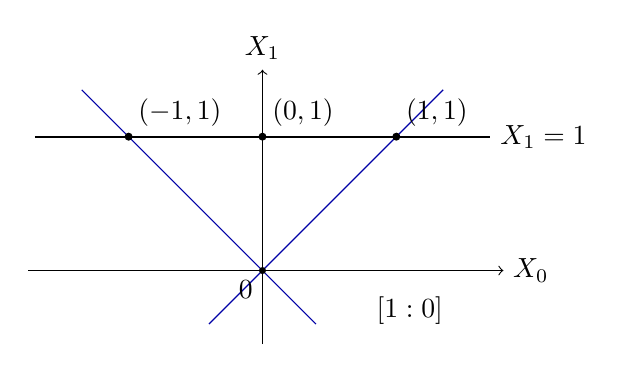
\begin{tikzpicture}[scale=0.85]
	\draw[->] (-3.5,0)--(3.6,0) node[right] {\(X_0\)};
	\draw[->] (0,-1.1)--(0,3) node[above] {\(X_1\)};
	\draw[thick] (-3.4,2)--(3.4,2) node[right] {\(X_1=1\)};
	\draw[blue!65!black] (-0.8,-0.8)--(2.7,2.7);
	\draw[blue!65!black] (0.8,-0.8)--(-2.7,2.7);
	\fill (0,0) circle(1.5pt) node[below left] {\(0\)};
	\foreach \x/\lab in {-2/{(-1,1)},0/{(0,1)},2/{(1,1)}}
	{\fill (\x,2) circle(1.7pt);\node[above right] at (\x,2) {\(\lab\)};}
	\node[below] at (2.2,-0.25) {\([1:0]\)};
\end{tikzpicture}
